%% LyX 2.0.5.1 created this file.  For more info, see http://www.lyx.org/.
%% Do not edit unless you really know what you are doing.
\documentclass[english]{article}
\usepackage[T1]{fontenc}
%\usepackage[latin9]{inputenc}
\usepackage{listings}
\usepackage{geometry}
\geometry{verbose,tmargin=2cm,bmargin=3cm,lmargin=2cm,rmargin=2cm}
\usepackage{amssymb}
\usepackage{graphicx}

\makeatletter

%%%%%%%%%%%%%%%%%%%%%%%%%%%%%% LyX specific LaTeX commands.
\newcommand{\noun}[1]{\textsc{#1}}

\makeatother

\usepackage{babel}
\begin{document}

\title{STNUM - TP3\\
Statistique Paramétrique}


\author{\noun{Juste Raimbault}}

\maketitle

\section{Comparaison des estimateurs du paramètre de position}


\paragraph{Question 2}

Une loi Gaussienne est symétrique par rapport à sa moyenne, donc $\theta=5$
ici.


\paragraph{Question 3.a.1}

Par définition, $\theta_{1}=(\frac{1}{i}\sum_{k=1}^{i}u_{i})_{1\leq i\leq n}$,
ainsi la composante $i$ de $\theta_{1}$ est la moyenne des $i$
premières composantes de $U$.

De même, $[\theta_{2}]_{i}$ est la médiane des $i$ premières composantes
de $U$.


\paragraph{Question 3.a.2}

L'instruction de type dans un plot permet de définir le type de tracé,
en l'occurence ici une ligne géométrique reliant les points de la
courbe.


\paragraph{Question 3.b}

On remarque sur les graphes que les estimateurs convergent rapidement
vers la valeur attendue du paramètre.

La matrice renvoyée correspond aux vecteurs $\theta_{1}$ et $\theta_{2}$
dans deux colonnes juxtaposées.


\paragraph{Question 3.c}

En lançant la fonction modifiée sur de très grandes valeurs de $n$,
on peut supposer que l'estimateur $\hat{\theta_{3}}$ n'est pas convergent,
comme le montre la figure ci-dessous ($n=100000$):

\hfill{}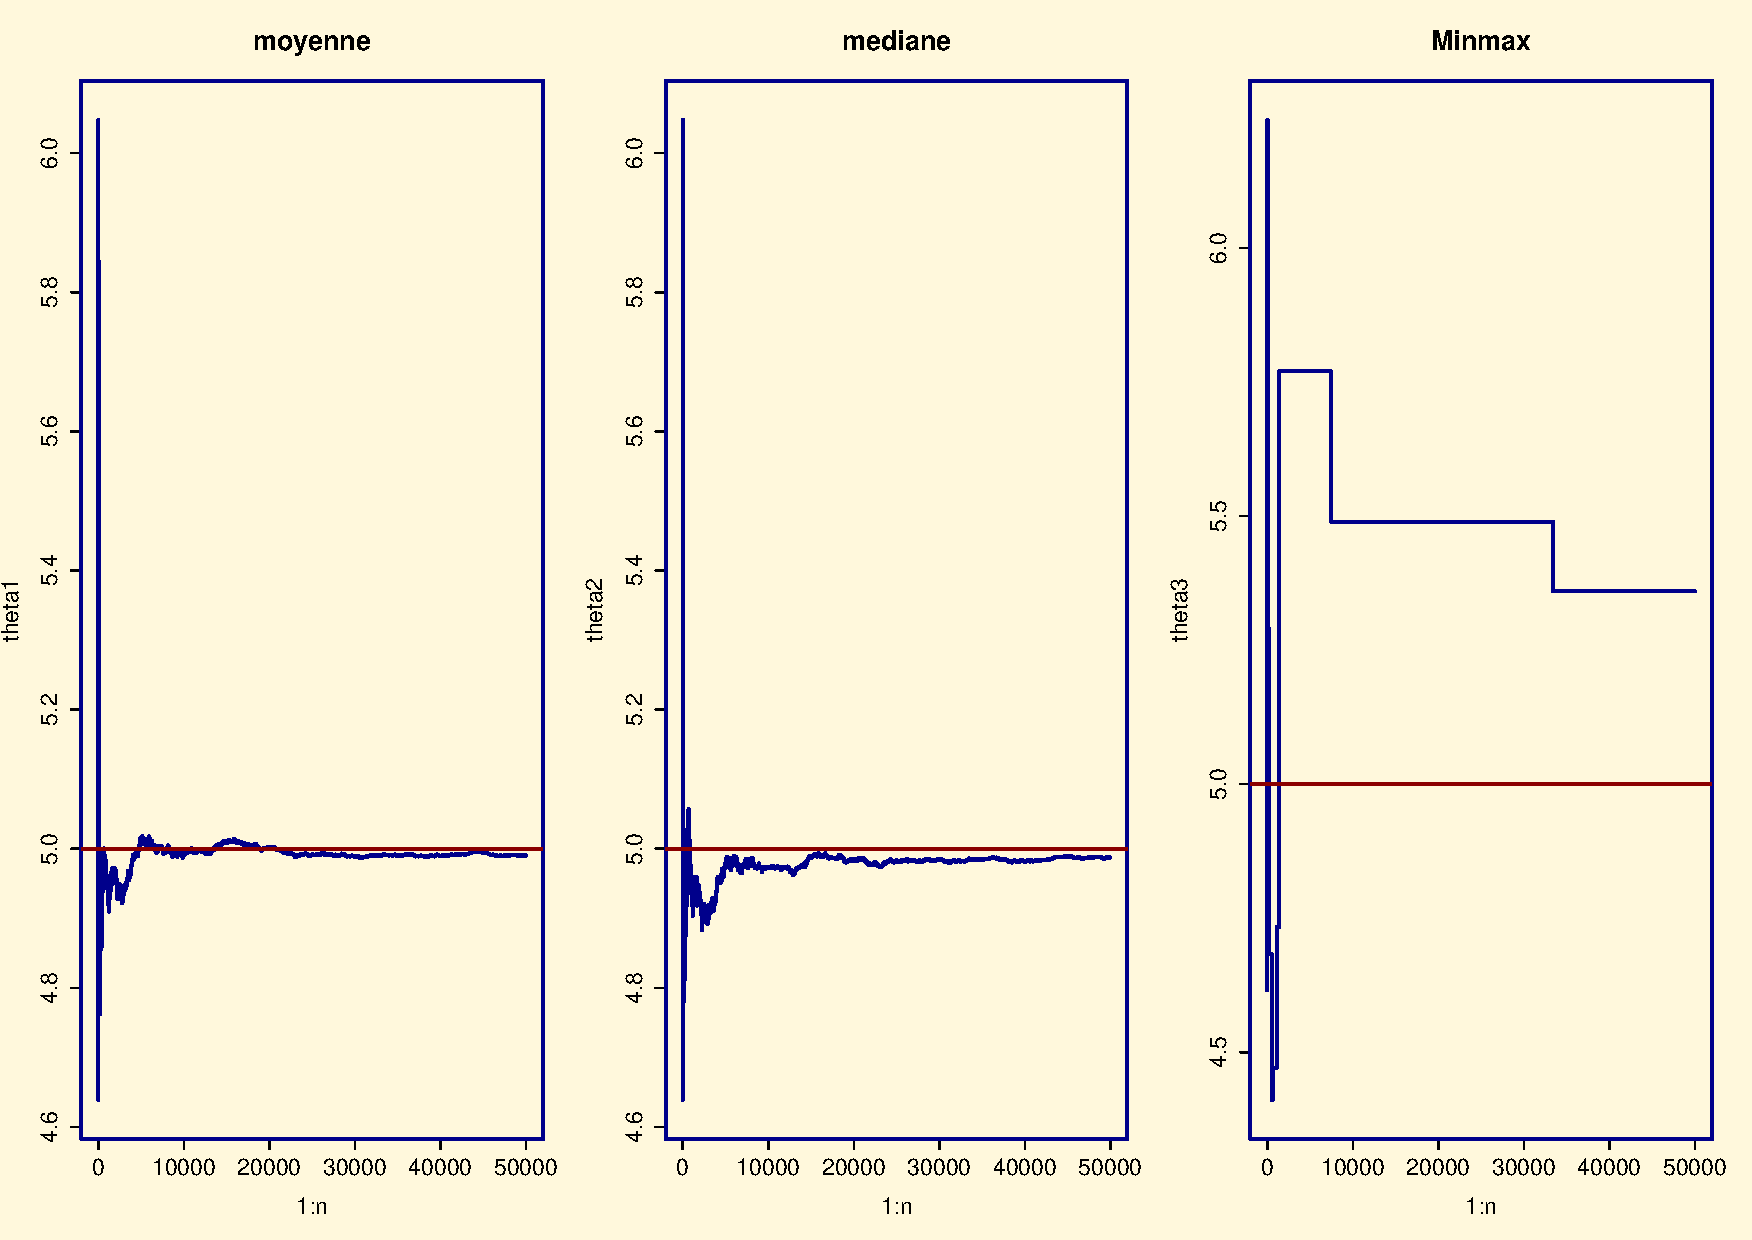
\includegraphics[scale=0.3]{convEstim}\hfill{}


\paragraph{Question 4.a}

La commande \texttt{apply} permet d'appliquer la fonction passée en
troisième argument aux sous-éléments de dimension le second argument
du tableau passé en premier argument. Dans notre cas, on applique
la fonction à chaque élément du vecteur.


\paragraph{Question 4.b}

On va préferer l'estimateur $\hat{\theta_{1}}$ au vu des boxplots
ci-dessous, car on préfère l'estimateur à moindre dispersion.

\hfill{}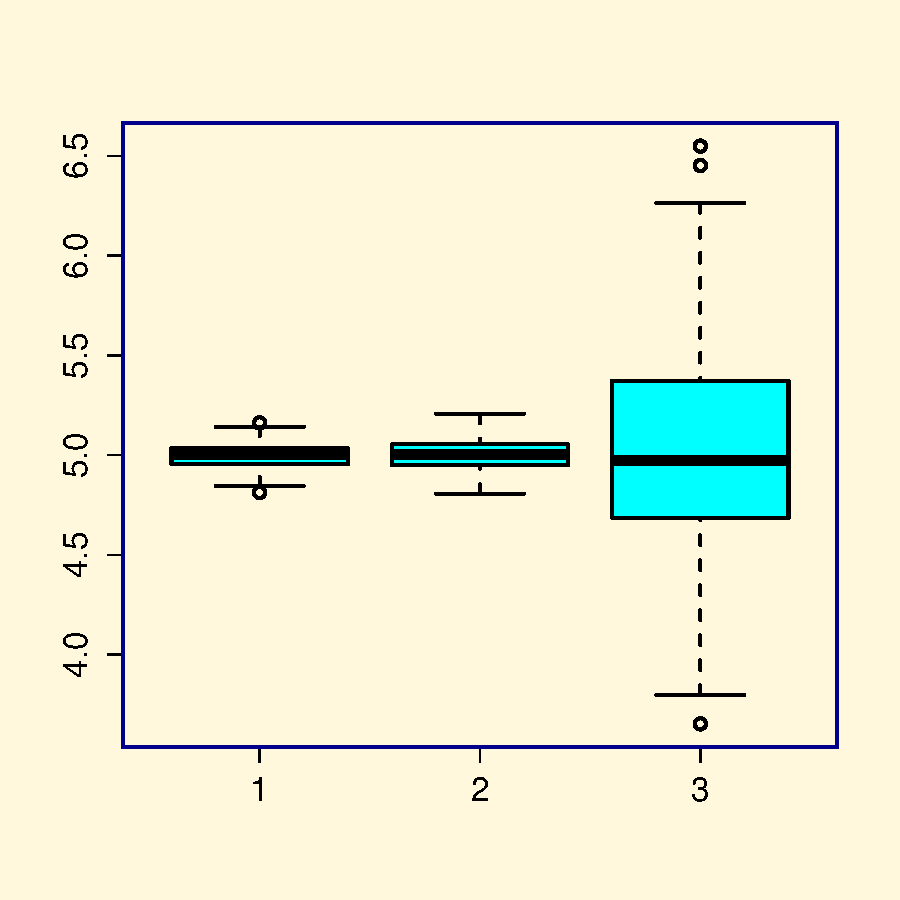
\includegraphics[scale=0.3]{boxCompEst}\hfill{}


\paragraph{Question 4.c}

Dans le cas de la loi uniforme, l'estimateur de loin le plus efficace
est $\hat{\theta_{3}}$ comme le montre le boxplot suivant. En effet,
une loi uniforme fournira intuitivement beaucoup plus rapidement le
min et le max plutôt qu'une moyenne ou une mediane stable.

\hfill{}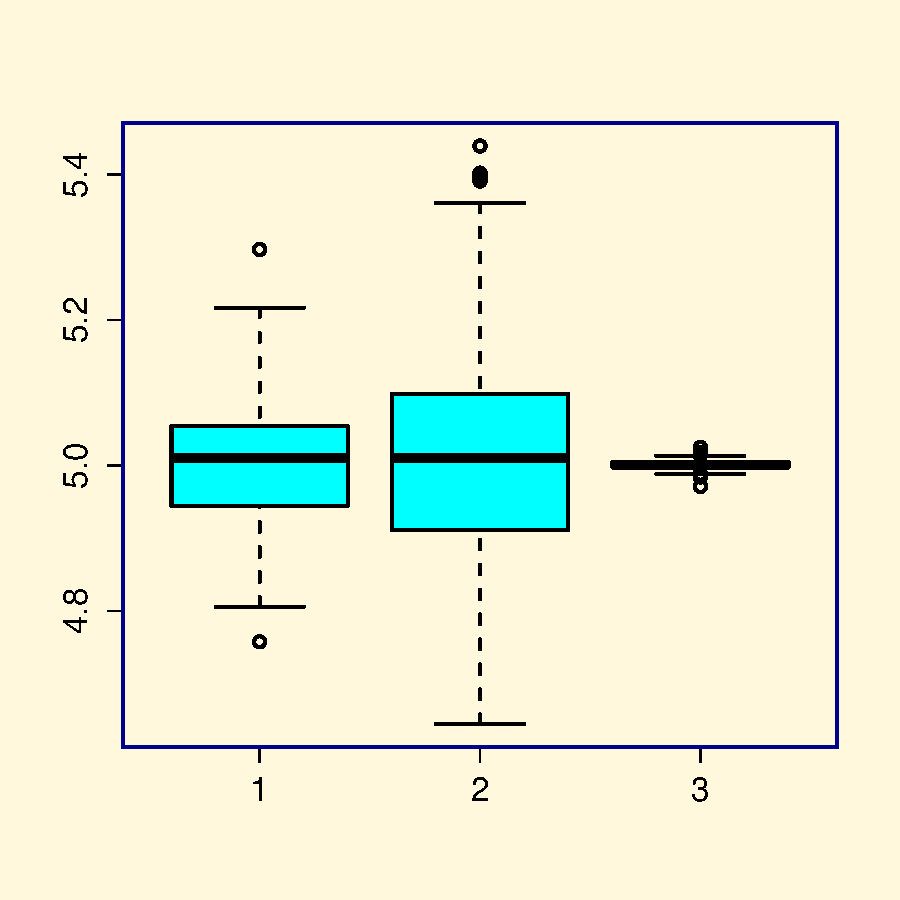
\includegraphics[scale=0.3]{EstUnif}\hfill{}


\paragraph{Question 4.d.i}

Enfin pour la loi de Cauchy, on s'aperçoit que $\hat{\theta_{3}}$
présente de très larges outliers et apparait assez inefficace (graphe
ci-dessous):

\hfill{}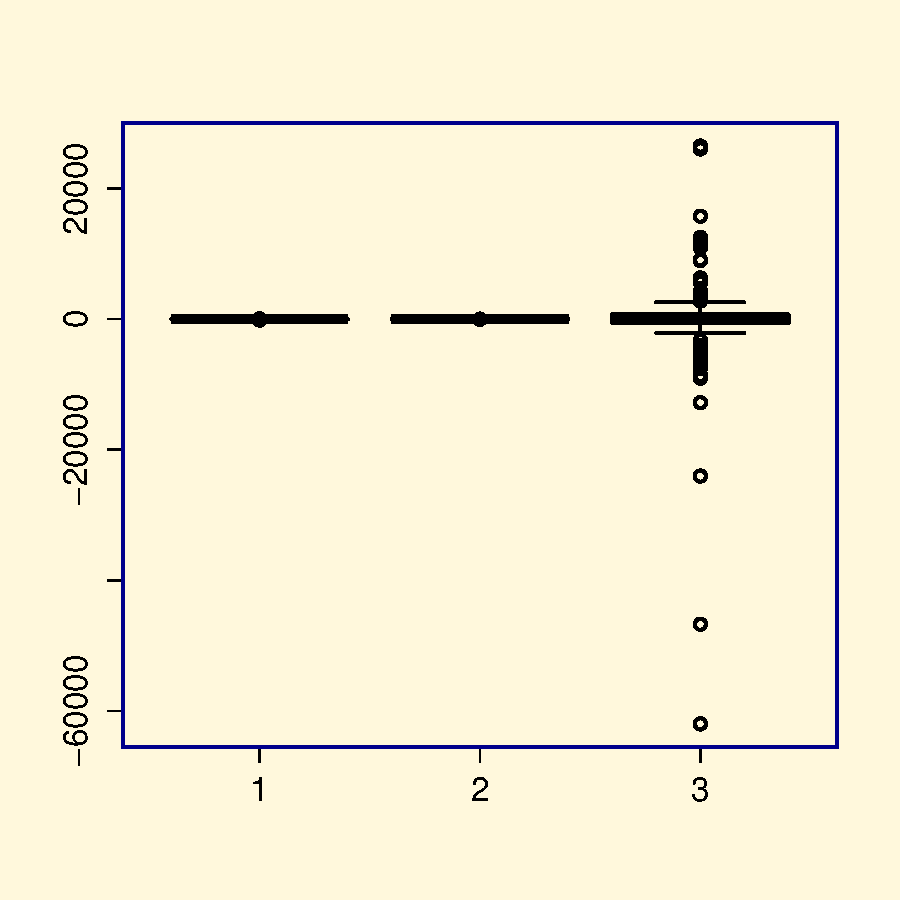
\includegraphics[scale=0.3]{EstCauchyTheta3}\hfill{}


\paragraph{Question 4.d.ii}

On relance sans le calcul de $\hat{\theta_{3}}$ our pouvoir comparer
$\hat{\theta_{1}}$ et $\hat{\theta_{2}}$. On peut conclure que la
médiane est bien meilleure car la distribution ne présente pas d'outliers
en comparaison avec la moyenne.

\hfill{}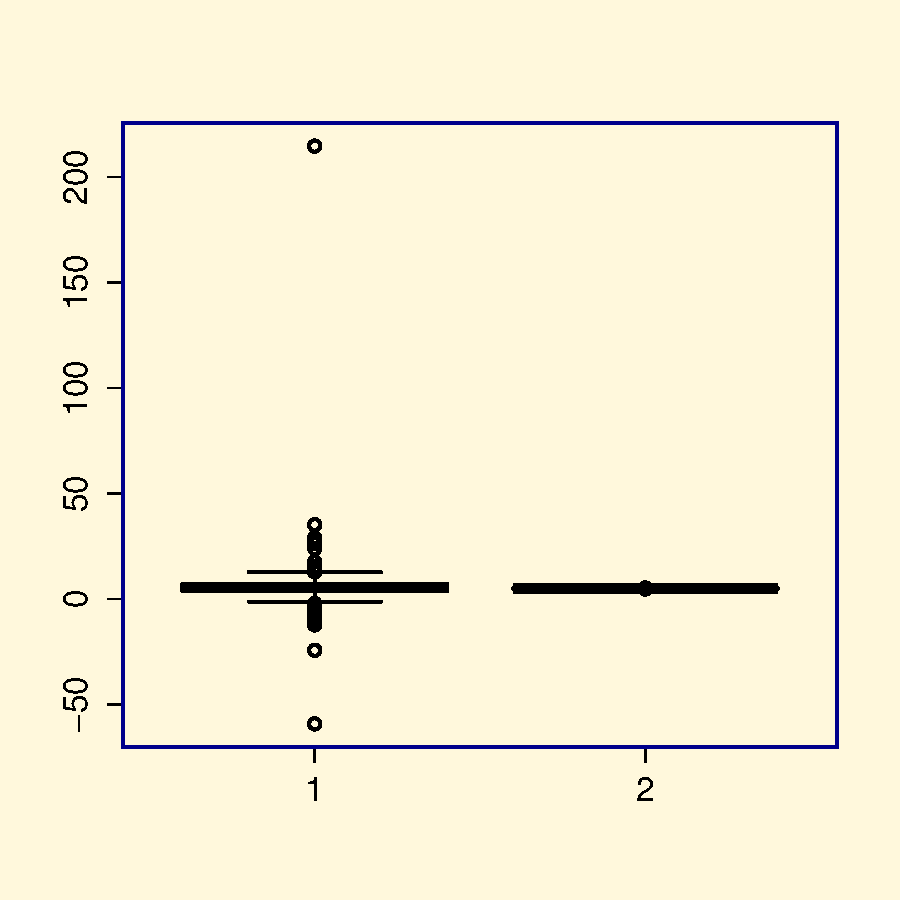
\includegraphics[scale=0.3]{EstCauchy2}\hfill{}

En conclusion, la loi normale a pour meilleur estimateur la moyenne,
la loi uniforme le min-max et la loi de Cauchy la médiane.


\paragraph{Question 5}

Comme on ne peut savoir a priori le type de loi, il faudrait lancer
chacun de ces trois estimateurs et supprimer incrémentalement le plus
mauvais jusqu'à obtenir un seul estimateur, qui correspondra a priori
à la loi de la distribution comme montré en 4 si cette loi existe.


\section{Intervalles de confiance (IC)}


\paragraph{Question 2.a}

On passe en argument à la fonction \texttt{quantile} les probabilités
0.025 et 0.975 pour avoir les quantiles voulus, qui sont de -1.897374
et 1.966214.


\paragraph{Question 2.b}

La distribution théorique attendue est ``normalisée'', i. e. ne
dépend pas de $\mu$ ni de $\sigma$, on s'attend à obtenir les mêmes
résultats, ce qu'on constate numériquement (avec des oscillations
qui ne dépassent pas celles observées à moyenne et écart-type fixés).


\paragraph{Question 2.c}

Augmenter $N$ ne change pas les résultats obtenus comme le montre
la courbe suivante pour le premier quantile par exemple, les fluctuations
étant uniquement aléatoires:

\hfill{}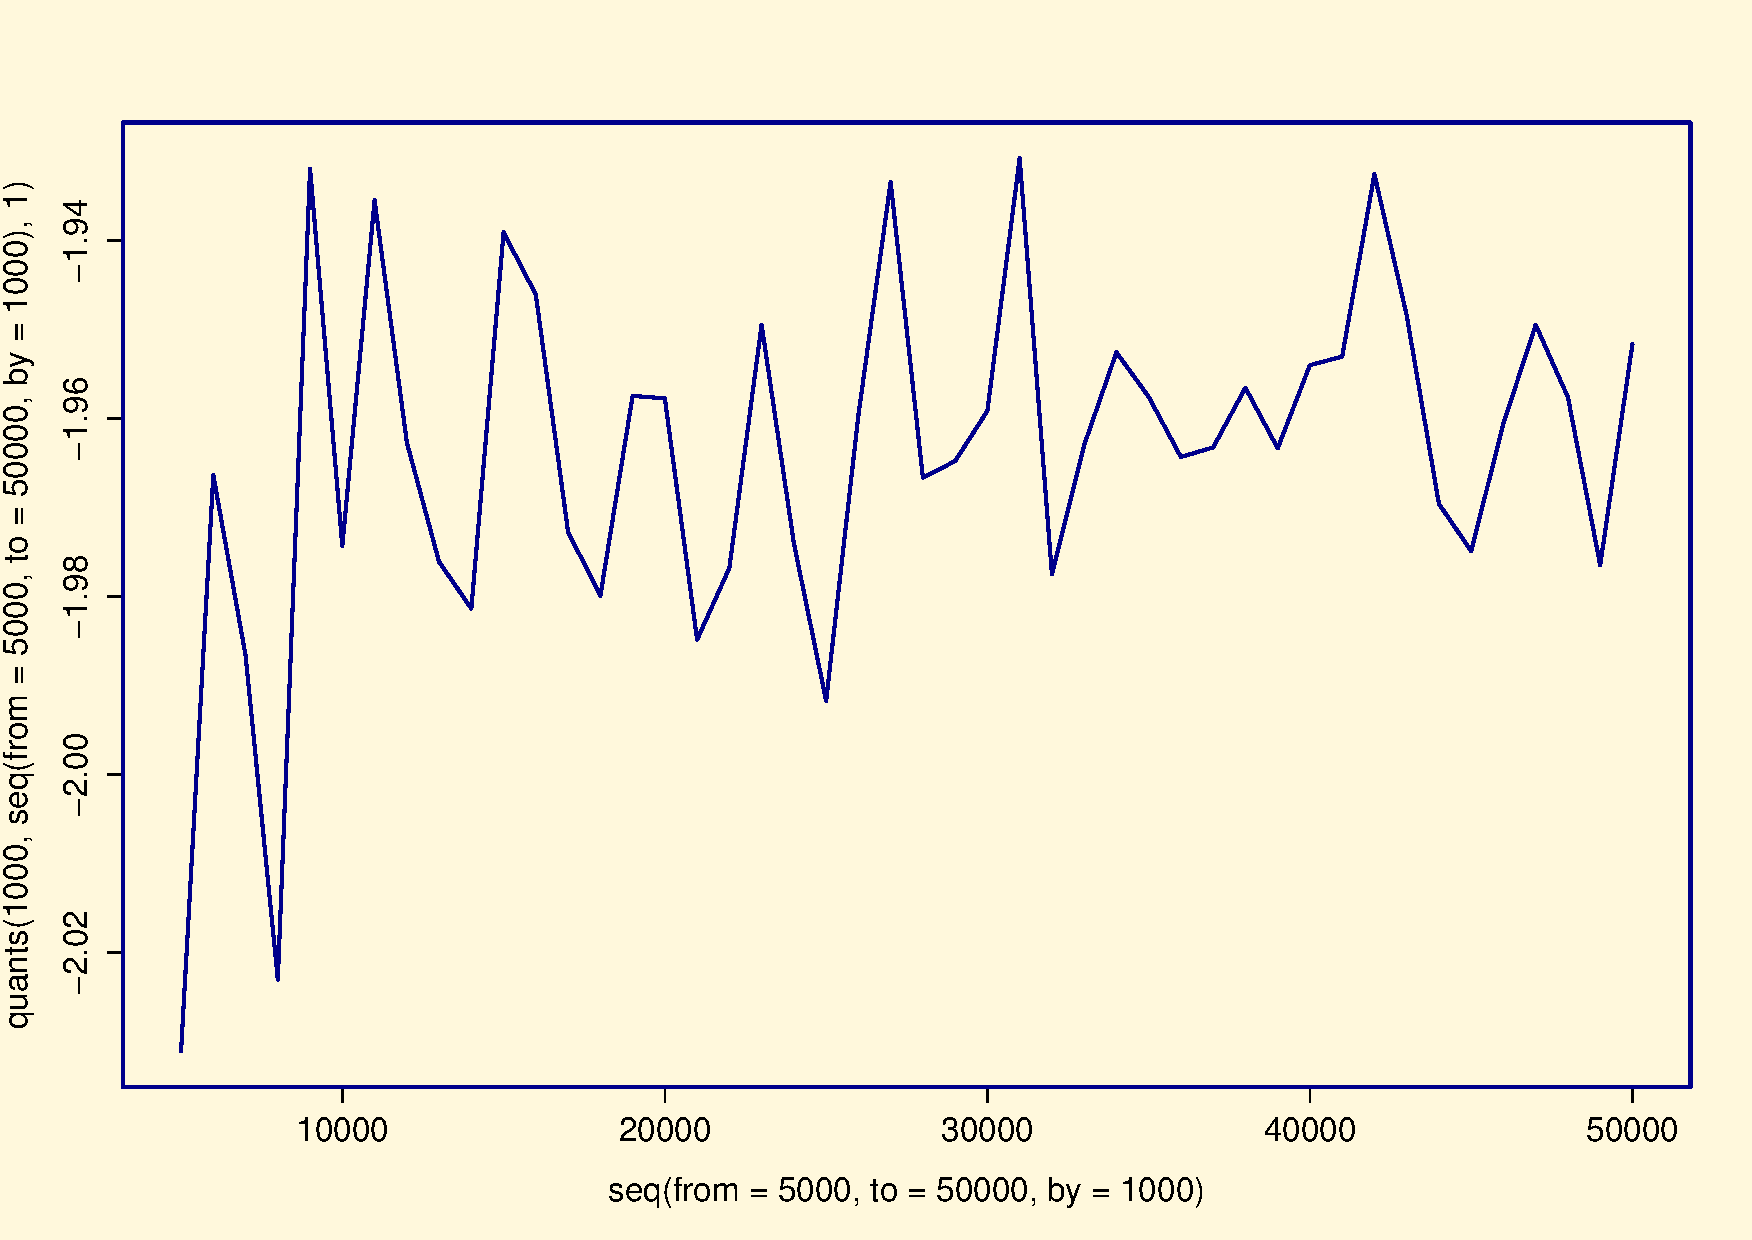
\includegraphics[scale=0.3]{firstquantile}\hfill{}


\paragraph{Question 2.d}

Par définition de $a$ et $b$, on a $\mathbb{P}(T<a)=0.025$ et $\mathbb{P}(T>b)=1-0.975=0.025$
donc $\mathbb{P}(T\in[a,b])=95\%$.


\paragraph{Question 2.e}

On a $T_{n}\in[a,b]\iff\frac{(\bar{X}-\mu)\sqrt{n}}{S_{n}}\in[a,b]\iff\bar{X}-\mu\in[\frac{S_{n}}{\sqrt{n}}a,\frac{S_{n}}{\sqrt{n}}b]\iff\mu\in[\bar{X}-\frac{S_{n}}{\sqrt{n}}b,\bar{X}-\frac{S_{n}}{\sqrt{n}}a]$,
d'où le résultat.

Par définition de l'intervalle de confiance, on a 95\% des échantillons
qui vérifient cette contrainte sur la moyenne.


\paragraph{Question 3.b}

On a $n=10$, et on obtient en utilisant la méthode précédente (quantiles
de la loi de student, avec $\mu$ moyenne de la série), $(a,b)=(-2.21,2.23)$.


\paragraph{Question 3.c}

On obtient l'intervalle de confiance pour la moyenne: $\mu\in[19.13,20.29]$.


\section{Calcul de l\textquoteright{}EMV à l\textquoteright{}aide de la commande
\texttt{mle}}


\paragraph{Question 2.a}

La commande \texttt{dgamma} calcule la valeur de la densité $p_{X}$
aux points du vecteur donné en argument, l'option \texttt{log=true}
permet d'obtenir $log(p_{X})$


\paragraph{Question 2.b}

Avec $a,\sigma>0$ et $X=(x_{i})_{1\leq i\leq n}$, on a $ll(a,\sigma)=-\sum_{i=1}^{n}log(p_{X}(x_{i},a,\sigma))=-log(\prod_{i=1}^{n}p_{X}(x_{i},a,\sigma))$


\paragraph{Question 2.c}

L'estimateur du maximum de vraissemblance est obtenu en minimisant
la fonction $ll$.


\paragraph{Question 3}

On obtient $a=8.39\pm1.64$ et $\sigma=6.19\pm1.25$.


\paragraph{Question 4}

L'IC de niveau 95\% pour $a$ est $[5.57,12.05]$. Celui de niveau
85\% pour $\sigma$ est $[4.27,9.48]$.


\paragraph{Question 5}

La surface a été transformée par la fonction $f(z)=log(0.001+\frac{z-z_{min}}{z_{max}-z_{min}})$
(on normalise pour avoir des valeurs entre 0.001 et 1.001 et on prend
le log). Sans la transormation, la surface est en majorité quasi-plate
et on ne peut visualiser correctement la position du minimum sur la
partie plate.


\paragraph{Question 6}

On obtient $a=5.14$ et $\sigma=2.88$ avec pour intervalles de confiance
à 95\% respectifs $[4.71,5.59]$ et $[2.64,3.16]$ ce qui est assez
proches des vraies valeurs.


\paragraph{Question 7}

On s'apercoit que le point obtenu est relativement constant lorsqu'on
fait varier les conditions initiales ($a=1,2,3,4;\sigma=1,2,3,4$),
par contre on obtient des points singuliers comme pour $\sigma=0.5$
pour lequel le résultat diverge.


\paragraph{Question 8.a}

On minimise la log-vraisemblance comme pour l'estimation des paramètres
de la loi gamma; la fonction est une adaptation de la fonction pour
la loi gamma.


\paragraph{Question 8.b}

Les estimations obtenues sont $a=6.53$ (IC $[3.65,9.39]$) et $s=10.14$
(IC $[7.68,13.41]$).


\paragraph{Question 8.c}

Pour $a>0,s>1$, le résultat obtenu semble être constant. Cela est
rendu possible car la fonction de log-vraissemblance est convexe pour
une loi de Cauchy, l'optimisation donne donc toujours le même point
sur cet ensemble.


\paragraph{Question 8.d}

On obtient la surface:

\hfill{}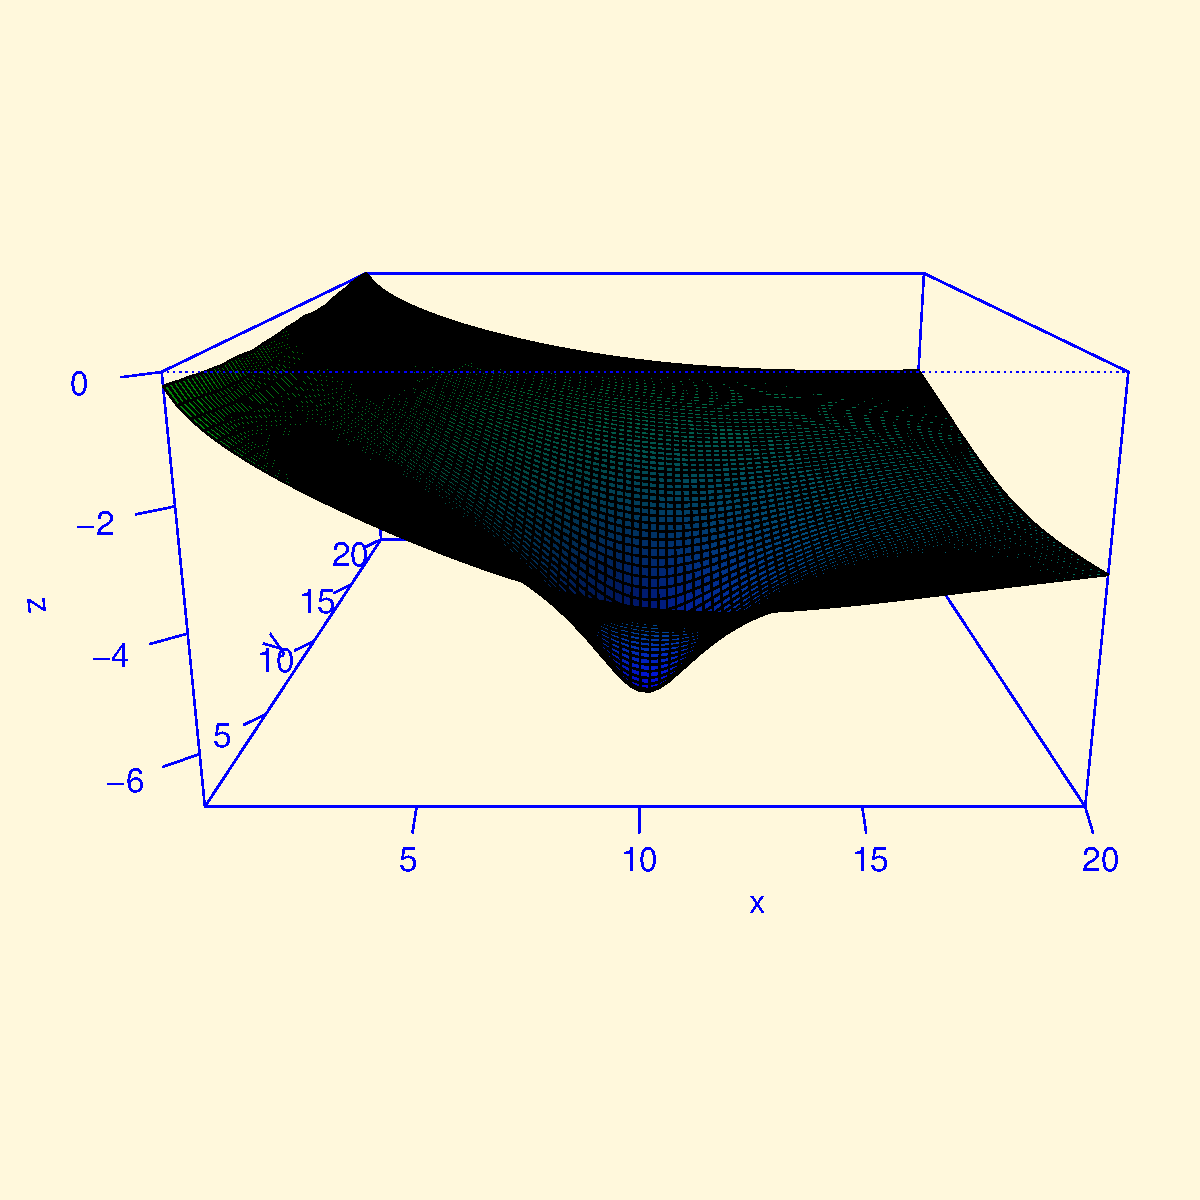
\includegraphics[scale=0.3]{3d}\hfill{}

\begin{lstlisting}[basicstyle={\tiny},numbers=left,numberstyle={\tiny},stepnumber=5]


#comparison of estimators for position parameter

n=10000;
X=rnorm(n,mean=5,sd=2);
par(bg="cornsilk",lwd=2,col="darkblue")
hist(X,breaks=40,freq=F,col="cyan")
curve(dnorm(x,mean=5,sd=2),add=T)


location_estimator=function(U,theta){
  n=length(U)
  theta1=cumsum(U)/(1:n)
  theta2=1:n;theta3=1:n;
  for (i in 1:n){
    theta2[i]=median(U[1:i])
    theta3[i]=(min(U[1:i])+max(U[1:i]))/2
  }
  par(mfrow=c(1,3),bg="cornsilk",lwd=2,col="darkblue")
  plot(1:n,theta1,type="l",main="moyenne")
  abline(h=theta,col="darkred")
  plot(1:n,theta2,type="l",main="mediane")
  abline(h=theta,col="darkred")
  plot(1:n,theta3,type="l",main="Minmax")
  abline(h=theta,col="darkred")
  #return(matrix(c(theta1,theta2,theta3),n,3))
}

location_estimator(rnorm(100000,mean=5,sd=2),5)

compare_estimators=function(N,n){
  par(mfrow=c(1,1))
  X=matrix(rcauchy(N*n,location=5,scale=2),N,n)
  theta1=apply(X,1,mean)
  theta2=apply(X,1,median)
  #theta3=(apply(X,1,min)+apply(X,1,max))/2
  par(bg="cornsilk",lwd=2,col="darkblue")
  boxplot(theta1,theta2,col="cyan")
}

compare_estimators(200,1000)




check_student=function(N,n,mu,sigma)
{
  X=matrix(rnorm(N*n,mean=mu,sd=sigma),N,n)
  t=sqrt(n)*(apply(X,1,mean)-mu)/apply(X,1,sd)
  return(t)
}

N=20000; n=1000;
t=check_student(N,n,100,50)
par(bg="cornsilk",lwd=2,col="darkblue")
hist(t,breaks=100,freq=F,col="cyan")
curve(dt(x,n-1),add=T,lwd=2)

quantile(x=t,probs=c(0.025,0.975))

quants = function(n,Nrange,ind){
  res=c()
  for(N in Nrange){
    res = append(res,quantile(x=check_student(N,n,100,50),probs=c(0.025,0.975))[[1]])
  }
  return(res)
}

plot(x=seq(from=5000,to=50000,by=1000),y=quants(1000,seq(from=5000,to=50000,by=1000),1),type="l")

X=c(19.6, 19.9, 20.4, 19.8, 20.5, 21.0, 18.5, 19.7, 18.4, 19.4)
n=10

mean(X) - quantile(x=check_student(20000,10,mean(X),sd(X)),probs=c(0.025,0.975)) * sd(X)/sqrt(10)


#X=c(77.551, 45.195, 50.626, 39.878, 29.137, 57.321, 39.140, 66.776, 48.028, 42.325, 31.200, 38.632, 42.914, 60.969, 22.076, 52.446, 45.257, 42.626, 62.504, 22.684, 69.196, 42.383, 61.339, 45.803, 74.707, 33.048, 72.423, 43.670, 65.279, 42.714, 59.785, 101.742, 59.641, 44.749, 44.161, 58.488, 46.448, 25.280, 67.619, 66.846, 80.208, 98.492, 41.149, 40.395, 22.220, 34.628, 77.768, 48.161,48.909, 66.267)

X = c(-7.54,  82.51,  14.27,   3.96,  189.98,   17.20,  -20.07,   52.66,   93.47,
-33.57,  13.13,  -1.26,  12.69,   53.33,    2.85,   -7.25,   13.30,   -5.67,
-38.99,  24.24,   4.17,  12.30,   21.59,   -6.70,    1.24,   13.91,   30.24,
3.35,   6.45, -26.22,  72.65,   10.12,   -1.64,   21.49,  391.11,   26.53,
146.60,   2.11,   5.84,  14.25,    7.17,    4.96,   -9.55,    7.89,   -2.31,
91.11,   8.39,   6.23,  25.45,    9.36,  102.44,   -7.28,  -40.02,   -8.86,
14.11,   6.84, -11.15,  -6.67,  -84.82, -241.41,   -0.14,  -72.95,   21.09,
53.47,  -3.80, -10.64,  19.71,   45.89, -124.30,   -2.02,   -1.67,    7.81,
-9.76,   6.25,  16.68,   8.88,   32.14,    1.29,  -10.00,   -5.03,  -66.77,
12.85,  15.32,  31.27,   6.59,    3.92,    8.61,   15.38,   -1.34,   14.11,
10.53,   2.35, -94.19,  16.45,    2.97,   12.26,    4.15,   10.63,    5.47)

ll=function(a=0.5, sigma=1.5)
{
  if(a > 0 && sigma > 0)
    -sum(dcauchy(X, location=a, scale=sigma, log=TRUE))
  else
    NA
}

library(stats4)
fit = mle(ll)
summary(fit)

vcov(fit)
par(mfrow=c(2,1),bg="cornsilk",col="blue",lwd=2)
plot(profile(fit), absVal=FALSE)
confint(fit,level=0.95)


# Calcul des valeurs de la log-vraisemblance
K=80
x=(1:K)/4;  y=(1:K)/4;  z=c();
for (i in 1:length(x))
  for (j in 1:length(y))
    z=c(z,ll(x[i],y[j]))
# Transformation des valeurs calculées
z=matrix(z,length(x),length(y))
z=log(0.001+((z-min(z))/(max(z)-min(z))))
# Le contenu des 7 lignes suivantes peut etre utilisé comme une
# boîte noire
nrz <- nrow(z)
ncz <- ncol(z)
jet.colors <- colorRampPalette( c("blue", "green") )
nbcol <- 100
color <- jet.colors(nbcol)
zfacet <- z[-1, -1] + z[-1, -ncz] + z[-nrz, -1] + z[-nrz, -ncz]
facetcol <- cut(zfacet, nbcol)
# Visualisation des résultats
par(bg="cornsilk",lwd=1,mfrow=c(1,1))
#image(x,y,z,col = cm.colors(50))
#contour(x,y,z,add=T,col="darkred")
persp(x, y, z,ticktype="detailed",expand=0.5,col=color[facetcol],shade=0.4)

X = rgamma(1000,shape=5,scale=3)
fit = mle(ll)
summary(fit)
confint(fit,level=0.95)



\end{lstlisting}

\end{document}
